\documentclass[12pt]{article}
\usepackage{amsmath}
\usepackage{array}
% \usepackage{gensymb}
\usepackage{geometry}
\usepackage{graphicx}
\usepackage{pgfplots}
\usepackage{siunitx}
\usepackage{wrapfig}

\title{Homework \#14}
\author{Donald Aingworth IV}
\date{November 27, 2024}

\pgfplotsset{width=8cm,compat=1.9}
\usepgfplotslibrary{external}
% \tikzexternalize

\begin{document}

\DeclareSIUnit{\mile}{mi}
\DeclareSIUnit{\gal}{gal}
\DeclareSIUnit{\foot}{ft}
\DeclareSIUnit{\h}{h}
\DeclareSIUnit{\rad}{rad}
\DeclareSIUnit{\u}{u}

\maketitle

\pagebreak

\section{Problem 1}
A wheel, whose moment of inertia is 0.0300 \unit{\kilo\gram*\meter^2}, is accelerated from rest to 20.0 rad/s in 5.00 s. When the external torque is removed, the wheel stops in 1 min. Find: (a) the frictional torque; (b) the external torque.

\subsection{Solution}
\subsubsection{Section (a)}
When only the frictonal torque is active, the radial velocty goes from 20 rad/s to 0 rad/s in 60 seconds. We can find the acceleration here by using a simple angular velocity formula.
\begin{align}
    \theta  &=  \theta_0 + \alpha t \rightarrow \alpha = \frac{\theta - \theta_0}{t}\\
    \alpha  &=  \frac{0 - 20}{60} = -\frac{1}{3}\unit{\rad/\second^2}
\end{align}

We now can use the formula for torque from angular acceleration to find the solution.
\begin{equation}
    \tau_{friction} =   I \alpha 
        = 0.030 * \left(-\frac{1}{3}\right) 
        = \boxed{0.010\unit{\newton\meter}}
\end{equation}

\subsubsection{Section (b)}
\begin{align}
    \alpha  &=  \frac{\theta - \theta_0}{t}
        =   \frac{20.0 - 0.0}{5.0}
        =   4.0 \unit{\second^{-2}}\\
    \tau_{net}  &=  I\alpha
        =   0.0300 * 4.0
        =   0.120 \unit{\newton\meter}
        =   \tau_{ext} + \tau_{friction}\\
    \tau_{ext}  &=  \tau_{net} - \tau_{friction}
        =   0.120 - 0.010
        =   \boxed{0.110 \unit{\newton\meter}}
\end{align}


\pagebreak

\section{Problem 2}
A block of mass m = 2.00 kg hangs vertically from a frictionless pulley of mass M = 4.00 kg and radius R = 15.0 cm. Find: (a) the acceleration of the block; (b) the tension in the rope; (c) the speed of the block after it has fallen 40.0 cm—assuming it started at rest. Treat the pulley as a solid disk.

\subsection{Solution}
\subsubsection{Section (a)}
We can start by creating an equation for the net vertical force on the block. There are two forces: the gravitational force and the tension force.
\begin{equation} F_{net} = T + F_g = T + mg = ma \end{equation}

We can next form the net rotational force on the pulley. To do this, we could calculate the torque of the disc. To do that, we would need to calculate the inertia of the pulley, which is the moment of inertia of a disc.
\begin{equation} I = \frac{1}{2}MR^2 \end{equation}

We here have two equations for torque, one from inertia \(\tau = I\alpha\), and one from force \(\tau = Fr\sin(\theta)\), with $\theta = \pi/2$ so $\sin(\theta) = 1$ since the force is downwards, perpendicular to the radius applied. We can combine these to get a formula for the force. and use that to get the net force and tension equation. We can also use $a = r\alpha$ to get $\alpha = \frac{a}{r}$, which we can use. 
\begin{align}
    I\alpha &=  Fr\\
    F_\tau  &=  \frac{MR^2}{2R}\alpha
        =   \frac{1}{2}Ma\\
    F_{net} &=  Ma
        =   F_\tau - T
\end{align}

We next can add equation (7) and equation (11) together to get a formula.
\begin{align}
    Ma + ma &=  \frac{1}{2}Ma - mg\\
    2Ma + 2ma   &=  Ma - 2mg\\
    (M + 2m)a   &=  2mg\\
    a   &=  \frac{2mg}{M + 2m}
\end{align}

\subsubsection{Section (b)}
We can substitute the acceleration into a formula including tension, in this instance \(ma = T + mg\).
\begin{align}
    T   &=  ma - mg
        =   \frac{2m^2g}{M + 2m} + mg
\end{align}

\subsubsection{Section (c)}
We have the acceleration and the change in position. We can apply this to a kinematic formula to get a final velocity.
\begin{align}
    v^2 &=  v_0^2 + 2a\Delta y
        =   \frac{4mg}{M + 2m}\Delta y
\end{align}

\pagebreak

\section{Problem 3}
\begin{wrapfigure}{r}{0.35\textwidth}
    \vspace{-30pt}
    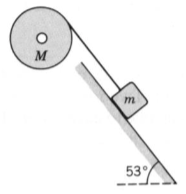
\includegraphics[width=0.35\textwidth]{graph_3.png} 
    % \label{fig:wrapfig}
\end{wrapfigure}
A block of mass m = 2.00 kg can slide down a frictionless 53\unit{\degree} incline, but it is connected to a pulley of mass M = 4.00 kg and radius R = 0.500 m, as shown in the figure below. The pulley can be treated as a disk. Find: (a) the angular acceleration of the pulley; (b) the speed of the block after it has slid 1.00 m, starting from rest.

\subsection{Solution}
\subsubsection{Section (a)}
First, there is the set of formulas for the torque, that we can combine. Since the pulley can be treated as a disc, we can use its formula for the moment of inertia \(I = \frac{1}{2}MR^2\).
\begin{align}
    I\alpha &=  F R\\
    F   &=  \frac{I\alpha}{R}
        =   \frac{1}{2}MR\alpha
\end{align}


\pagebreak

\section{Problem 4}
A car is traveling at 75.0 km/h has tires of 70.0 cm diameter. (a) What is the angular velocity of the tires about their axles? (b) If the car is brought to a stop uniformly in 30.0 complete turns of the tires (without skidding), what is the magnitude of the angular acceleration of the wheels? (c) How far does the car move during the braking?

\subsection{Solution}


\pagebreak

\section{Problem 5}
\begin{wrapfigure}{r}{0.35\textwidth}
    \vspace{-30pt}
    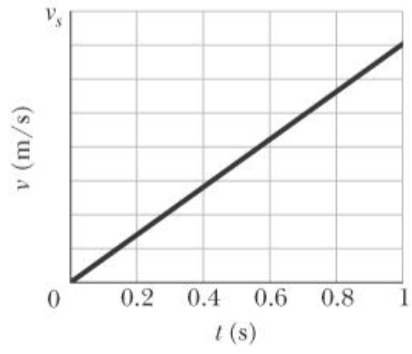
\includegraphics[width=0.35\textwidth]{graph_5.png} 
    % \label{fig:wrapfig}
\end{wrapfigure}
The graph below shows the speed v versus time t for a 0.500 kg object of radius 6.50 cm that rolls smoothly down a 30\unit{\degree} ramp. The scale on the velocity axis is set by vs = 4.0 m/s. What is the rotational inertia of the object?

\subsection{Solution}


\pagebreak

\section{Problem 6}
A hollow sphere of radius 0.15 m, with rotational inertia I = 0.040 kg · m2 about a line through its center of mass, rolls without slipping up a surface inclined at 30° to the horizontal. At a certain initial position, the sphere's total kinetic energy is 20 J. (a) How much of this initial kinetic energy is rotational? (b) What is the speed of the center of mass of the sphere at the initial position? When the sphere has moved 1.0 m up the incline from its initial position, what are (c) its total kinetic energy and (d) the speed of its center of mass?

\subsection{Solution}


\pagebreak

\section{Problem 7}
A yo-yo has a rotational inertia of 900 g · cm2 and a mass of 100 g. Its axle radius is 3.2 mm, and its string is 120 cm long. The yo-yo rolls from rest down to the end of the string. (a) What is the magnitude of its linear acceleration? (b) How long does it take to reach the end of the string? As it reaches the end of the string, what are its (c) linear speed, (d) translational kinetic energy, (e) rotational kinetic energy, and (f) angular speed?

\subsection{Solution}


\pagebreak

\section{Problem 8}
\begin{wrapfigure}{r}{0.35\textwidth}
    \vspace{-30pt}
    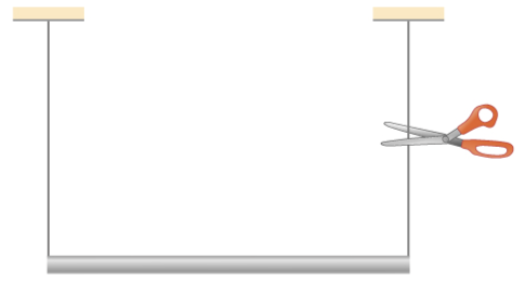
\includegraphics[width=0.35\textwidth]{graph_8.png} 
    % \label{fig:wrapfig}
\end{wrapfigure}
A uniform rod is held vertically by two strings of negligible mass, as shown below. (a) Immediately after the string is cut, what is the linear acceleration of the free end of the stick? (b) Of the middle of the stick?

\subsection{Solution}


\end{document}